% Generated by ICLR_Q4.py from experiment_logs_Q4 -- Dubins4D_x0set: Total runtime [s]
% Shaded band = min/max over seeds; line = median over seeds.
% Picture width is exactly \linewidth. Requires \usepackage{pgfplots}.
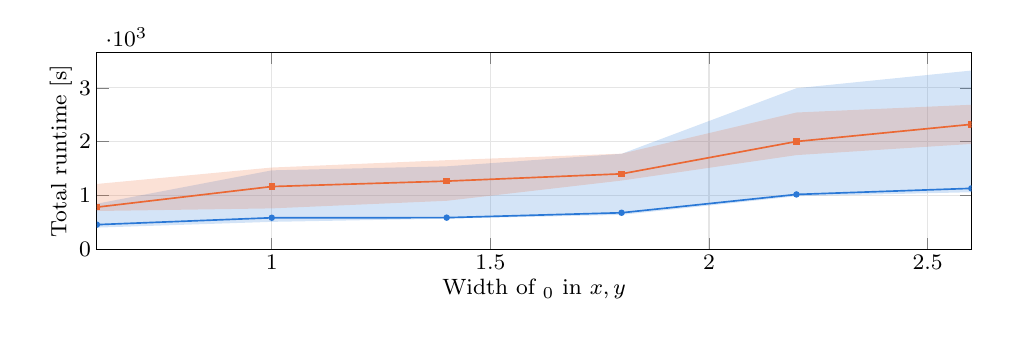
\begin{tikzpicture}[baseline=(current axis.south)]
\definecolor{q4ppo}{RGB}{42,120,214}
\definecolor{q4sac}{RGB}{235,104,52}
\begin{axis}[
    scale only axis, width=\linewidth-25pt-4pt, height=2.5cm,
    xlabel={Width of $\X_0$ in $x,y$},
    ylabel={Total runtime [s]}, ylabel style={align=center},
    xmin=0.6, xmax=2.6, xtick={1,1.5,2,2.5},
    ymin=0, scale ticks above exponent=2,
    grid=major, grid style={gray!20}, clip marker paths=true,
    label style={font=\footnotesize}, tick label style={font=\footnotesize, inner sep=2pt},
    xlabel shift=-2pt, ylabel shift=-3pt,  % labels close to the tick labels
]
% PPO: 5 seeds per X0 span
\addplot[draw=none, fill=q4ppo, fill opacity=0.2, forget plot] coordinates {(0.6,406.064) (1,512.852) (1.4,572.495) (1.8,643.146) (2.2,989.228) (2.6,1062.94) (2.6,3322.39) (2.2,2994.06) (1.8,1776.63) (1.4,1543.97) (1,1469.31) (0.6,850.361)} -- cycle;
\addplot[q4ppo, semithick, mark=*, mark size=0.85pt] coordinates {(0.6,461.161) (1,588.909) (1.4,591.171) (1.8,681.992) (2.2,1021.92) (2.6,1134.71)};
% SAC: 2/5 seeds per X0 span
\addplot[draw=none, fill=q4sac, fill opacity=0.2, forget plot] coordinates {(0.6,714.38) (1,762.866) (1.4,903.901) (1.8,1279.64) (2.2,1752.27) (2.6,1959.67) (2.6,2686.85) (2.2,2543.19) (1.8,1779.01) (1.4,1658.06) (1,1521.47) (0.6,1216.62)} -- cycle;
\addplot[q4sac, semithick, mark=square*, mark size=0.85pt] coordinates {(0.6,785.94) (1,1168.54) (1.4,1269.21) (1.8,1404.51) (2.2,2004.95) (2.6,2323.26)};
\end{axis}
% Fix the bounding box to exactly \linewidth wide: the axis box plus the label margins
\path (current axis.south west |- current bounding box.south) ++(-25pt,0) coordinate (q4sw)
      (current axis.north east |- current bounding box.north) ++(4pt,0) coordinate (q4ne);
\pgfresetboundingbox
\useasboundingbox (q4sw) rectangle (q4ne);
\end{tikzpicture}%
